\newpage
\section{Original Design Document}
\def\DDtitle{Computer Science Senior Software Engineering Project (CS462)}
\def\DDterm{Winter 2017}
	\begin{center}
		\vspace{\fill}

		{\Huge\bfseries Original Design Document\par}
		\vspace{0.5cm}
		{\Large\itshape \DDtitle\par}
		\vspace{0.5cm}
		{\Large\itshape \DDterm\par}
		
		\vspace{\fill}
	\end{center}
	\begin{abstract}
		A Head-up Display (HUD) Alignment system is developed as a proof of concept aims to explore a potential technological innovation for the HUD system that presents critical flight information to pilots. The primary objective of this project is to reduce the cost and time required to precisely align flight information to the HUD by introducing an additional sensor component to the system to make the alignment process more dynamic. This document is intended for use by Rockwell Collins and their HUD system development team. This document provides and explains an overall system framework, design viewpoints and specific design description for each viewpoint within the system.
	\end{abstract}
	
	\includepdf[pages=-]{pdf/design_doc.pdf}

\newpage
	\subsection{Necessary Change Based on Original Design}
		\subsubsection{Change in IV.COMSITION VIEW}
			\textbf{Hardware Configuration Design}
			\\ \indent The original diagram showed that the Aircraft IMU outputs aligned raw data to the microcontroller; what we did was both IMU would only output raw data and the alignment is measured/calculated by the microcontroller as figure~\ref{fig:hardware_config}.\\

			\begin{figure}
		 		\caption{New Data Flow diagram (Hardware)}
		      	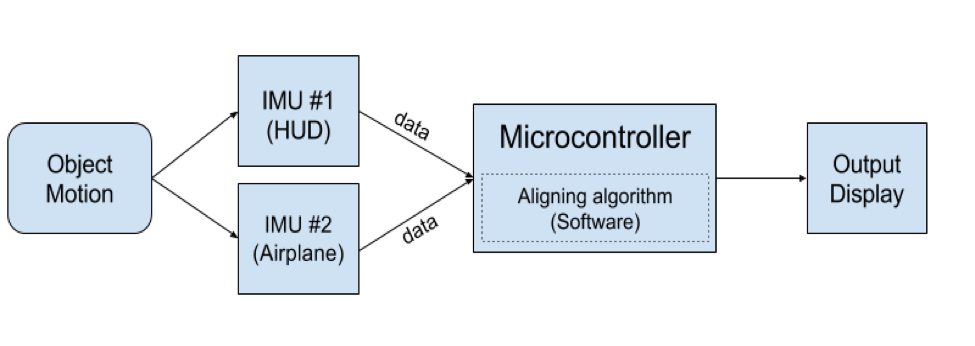
\includegraphics[width=\textwidth,height=\textheight,keepaspectratio]{hardware_config}
			    \label{fig:hardware_config}
			\end{figure}

		\subsubsection{Change In VI.INTERFACE VIEW}
			\textbf{Software User Interface Design}
			\\ \indent Our previous GUI have a 2D gauge-like looks to it. It looks more like a car dashboard rather than a real plane HUD. This GUI serve our purpose of showing the data well. However, it is hard to visualize the change on the plane for each angle. Our team is determined to give the best for this project and decided to improve on our GUI. To solve this problem, we create a new GUI as figure~\ref{fig:gui}  that visualize the change of angle to a plane object. We create this GUI by using a python sublanguage called VPython. We also use the pySerial library to connect the GUI to the Arduino part of the project.\\

			\begin{figure}
		 		\caption{New GUI by Vpython}
		      	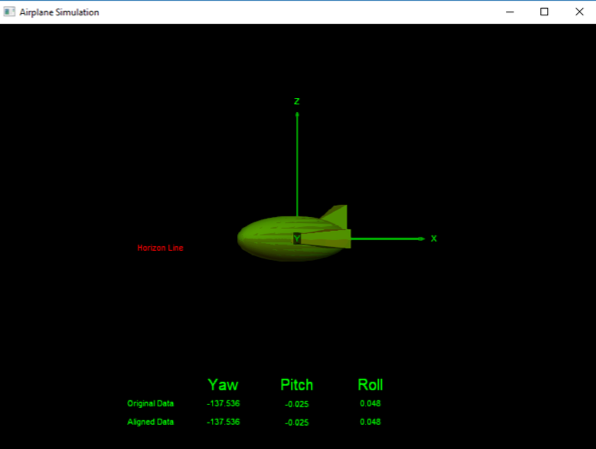
\includegraphics[width=\textwidth,height=\textheight,keepaspectratio]{gui}
			    \label{fig:gui}
			\end{figure}

		\subsubsection{Change In VIII Algorithm View}
			\textbf{Statistical Analysis Method for Initial Alignment Offset Design \& Offset Algorithm Design}
			\\ \indent For our statistical analysis, we applied a 95\% confidence interval to our offset data to ensure that the resulting offset was precise. By using a confidence interval, we can retrieve a valid offset value as soon as the quaternion value converges. Without using a confidence interval, we could end up with an erroneous value.

			Our implementation originally stored 60 samples each for the yaw, pitch and roll offset before using those values to find the confidence interval. Unfortunately, the microcontroller's memory is limited, which makes finding a precise value difficult. We were able to increase the number of samples and increase our performance by taking the offsets of each yaw, pitch and roll sequentially, thus tripling our sample sizes.

			Currently, the confidence interval is only being applied to the offsets between each device. Further improvements may be gained by increased use of statistical analysis. One such improvement would be to apply our analysis during calibration. The current process relies on a simple average of a single stream of data.











